\documentclass{exam} % {{{1
\usepackage{amsmath, amssymb, amsthm, enumitem, float, caption, mathtools, tikz}
\usetikzlibrary{arrows.meta, calc, decorations.markings, matrix, positioning}
\tikzset{>=latex}
\usepackage[final]{hyperref}

% mathbb and mathcal symbols
\newcommand{\NN}{\mathbb{N}}
\newcommand{\ZZ}{\mathbb{Z}}
\newcommand{\QQ}{\mathbb{Q}}
\newcommand{\RR}{\mathbb{R}}
\newcommand{\V}{\mathcal{V}}
\newcommand{\A}{\mathbb{A}}
\newcommand{\m}[1]{\mathbb{#1}}    % for models
\newcommand{\cl}[1]{\mathcal{#1}}  % for classes

% theorems and similar environments
\theoremstyle{plain}
  \newtheorem{thm}{Theorem}[section]  \newtheorem*{thm*}{Theorem}
  \newtheorem{claim}[thm]{Claim}      \newtheorem*{claim*}{Claim}
  \newtheorem{conj}[thm]{Conjecture}  \newtheorem*{conj*}{Conjecture}
  \newtheorem{cor}[thm]{Corollary}    \newtheorem*{cor*}{Corollary}
  \newtheorem{lem}[thm]{Lemma}        \newtheorem*{lem*}{Lemma}
  \newtheorem{prop}[thm]{Proposition} \newtheorem*{prop*}{Proposition}
\theoremstyle{definition}
  \newtheorem{defn}[thm]{Definition} \newtheorem*{defn*}{Definition}
  \newtheorem{ex}[thm]{Example}      \newtheorem*{ex*}{Example}
\theoremstyle{remark}
  \newtheorem{rk}[thm]{Remark}  \newtheorem*{rk*}{Remark}
\newcommand{\Case}[1]{\smallskip \textbf{Case #1:}}
\newenvironment{claimproof} {
  \begin{proof}[Proof of claim]
  \renewcommand{\qedsymbol}{\ensuremath{\bullet}}
  } {
  \end{proof}
  }

% custom commands
\DeclareMathOperator{\Cg}{Cg}
\DeclareMathOperator{\Clo}{Clo}
\DeclareMathOperator{\Con}{Con}
\DeclareMathOperator{\Rel}{Rel}
\DeclareMathOperator{\Sg}{Sg}
\DeclareMathOperator{\diag}{diag}
\newcommand{\bmat}[1]{ \begin{bmatrix} #1 \end{bmatrix} }
\newcommand{\Bmat}[1]{ \begin{Bmatrix} #1 \end{Bmatrix} }
\newcommand{\pmat}[1]{ \begin{pmatrix} #1 \end{pmatrix} }
\newcommand{\mat}[1]{ \begin{matrix} #1 \end{matrix} }
\newcommand{\vect}[1]{ \left< #1 \right> }
\newcommand{\ds}[1]{ \displaystyle{#1} }
\newcommand{\stack}[2]{\genfrac{}{}{0pt}{}{#1}{#2}}

% misc
\pagestyle{foot} \cfoot{Page \thepage}  % page numbering
\numberwithin{equation}{section}  % number equations within sections
\renewcommand{\d}{\;d}
\renewcommand{\epsilon}{\varepsilon}
\renewcommand{\phi}{\varphi}
\newcommand{\TODO}[1]{\noindent\textbf{TODO: #1}}

% exam documentclass settings
% restyle parts and subparts
\renewcommand{\thepartno}{\roman{partno}}
\renewcommand{\thesubpart}{\alph{subpart}}
\renewcommand{\subpartlabel}{(\thesubpart)}
\renewcommand{\subsubpartlabel}{(\thesubsubpart)}
% restyle multiple choice options
\renewcommand{\choicelabel}{\thechoice)}
% true or false questions (use \TFQuestion)
\newcommand{\TrueFalse}{\hspace*{0.25em}\textbf{True}\hspace*{1.25em}\textbf{False}\hspace*{1em}}
\newlength{\mylena} \newlength{\mylenb} \settowidth{\mylena}{\TrueFalse}
\newcommand{\TFQuestion}[1]{
  \setlength{\mylenb}{\linewidth} 
  \addtolength{\mylenb}{-121.15pt}
  \parbox[t]{\mylena}{\TrueFalse}\parbox[t]{\mylenb}{#1}
}

% document specific stuff
\newcommand{\sol}{\begin{center}\textbf{SOLUTION}\end{center}} 
%----------------------------------------------------------------------------}}}1

\begin{document}  % \printanswers
% title header {{{
\title{Quantum Algorithms \\ Homework 3 Solutions}
\author{Patrick Canny}
\date{Due: 2019-02-19}
\maketitle
%----------------------------------------------------------------------------}}}
\section{Book Problems}
\begin{questions}
%----------------------------------------------------------------------------}}}
  \question Exercise 3.3\\
  (Paraphrased)
  Suppose we have some NP-Oracle. Prove that there is a poly-time algorithm that
  finds a satisfying assignment for a given formula by making a polynomial number
  of queries to the oracle.\\
  \sol
  To solve this problem, I initially thought that it would be a good idea to start
  with an assignment of the input variables for a predicate, making them all False
  or something, and then going through the predicate clause-by-clause in order to 
  set and eliminate possibilities for each variable one at a time. After some thought,
  I discovered that this solution was actually an exponential time solution, as 
  some backtracking would need to occur if an assignment was incorrect, and there was
  no limit on the number of times that this backtracking would need to occur.\\

  The actual solution is the opposite procedure really: start with a given 
  predicate and ask the Oracle if it is satisfiable. If it is, then assign one of
  the variables as False and ask the Oracle if the original predicate can be
  satisfied with this given assignment. If it can't, then flip the variable's 
  value. If it can, then this assignment of the variable  is valid in the solution. 
  Repeat this procedure until all variables in the original predicate have a 
  valid assignment.\\

  This procedure is polynomial in the number of calls to the Oracle since the 
  Oracle will be invoked at most $1+k$ times, where $k$ is the number of
  input variables since the Oracle will be invoked once per input variable
  and an additional time at the beginning of the procedure.\\
%----------------------------------------------------------------------------}}}
  \question Exercise 3.6(a)\\
  Construct a polynomial reduction of 3-SAT to 3-Color\\
  \sol
  In order to create this polynomial reduction, we have to show in some way that
  a 3-SAT problem can be represented a 3-color problem. This can be done fairly 
  easily by using the nodes of the graph as variables and the edges as their 
  relationships to one another. We will then invoke new nodes to represent the
  True/False values of the results of these clauses. The following graph can be
  constructed as follows:
  \begin{center}
  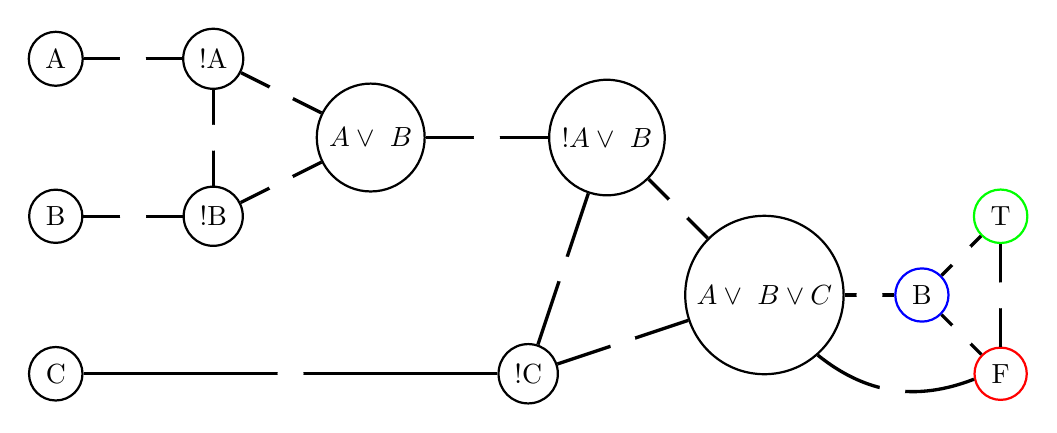
\begin{tikzpicture}
    \begin{scope}[every node/.style={circle,thick,draw}]
      \node (A) at (0,0) {!A};
      \node (B) at (0,-2) {!B};
      \node (C) at (4,-4) {!C};
      \node (G) at (-2,0) {A};
      \node (H) at (-2,-2) {B};
      \node (I) at (-2,-4) {C};
      \node (D) at (2, -1) {$A\lor\ B$};
      \node (J) at (5, -1) {!$A\lor\ B$};
      \node (E) at (7, -3) {$A\lor\ B \lor C$};
      \node[draw = blue] (X) at (9, -3) {B};
      \node[draw = green](T) at (10, -2) {T};
      \node (F)[draw = red] at (10, -4) {F};
    \end{scope}
    \begin{scope}[>={},
                  every node/.style={fill=white,circle},
                  every edge/.style={draw=black, very thick}]
      \path [->] (A) edge node {} (B);
      \path [->] (G) edge node {} (A);
      \path [->] (H) edge node {} (B);
      \path [->] (I) edge node {} (C);
      \path [->] (B) edge node {} (D);
      \path [->] (A) edge node {} (D);
      \path [->] (D) edge node {} (J);
      \path [->] (C) edge node {} (J);
      \path [->] (C) edge node {} (E);
      \path [->] (J) edge node {} (E);
      \path [->] (E) edge node {} (X);
      \path [->] (X) edge node {} (T);
      \path [->] (X) edge node {} (F);
      \path [->] (E) edge[bend right=30] node {} (F);
      \path [->] (T) edge node {} (F);
    \end{scope}
  \end{tikzpicture}
  \end{center}
  This graph will need to be constructed for each and every clause in the initial
  instance of 3-SAT.\\

  Now to show that this instance of 3-SAT is satisfiable, we have to show that the 
  graph above is 3-Colorable.\\

  First suppose that the instance is satisfiable. For every variable $v_i$ that
  is False, color that node on the graph the same color as node $F$, and go 
  through a similar process for the True variables. In order for this graph
  to be 3-Colorable, one of the input variables must be the True color. This
  is because the node $A\lor B \lor C$ must be a different color from the base 
  color (The arbitrary 3rd color of $X$) and the False color. If this is not 
  possible, the graph is not 3-colorable for the clause, and thus is not satisfiable
  for the whole 3-SAT instance.\\
  
  These graphs will need to be made for each clause in the given 3-SAT predicate,
  and the $A \lor B \lor C$ nodes for each graph will need to be connected to the
  base and false colors in the same way as the graph above.\\

  This is enough to show that 3-SAT can be reduced to 3-Color.
\end{questions}
%----------------------------------------------------------------------------}}}
\section{Additional Problems}
\begin{questions}
% Fermat's theorem   {{{1
\question Compute $\ds{ 2^{3^{4^5}} \bmod 79}$. If you use a computer to do
this, submit your code. There is a way to do this by hand that will almost
certainly be faster than a computer, however. [\emph{Hint: $78 = 2\cdot
3\cdot 13$.}] 
  \sol
  $\ds{ 2^{3^{4^5}} \bmod 79}$ can be solved using the following process:\\
  Examine \[\ds{3^{4^5}} \bmod 79 = l + k(78)\] which implies 
  \[ 2^l*(2^{78})^k = 2^l*(1)^k = 2^l \bmod 79 \]
  from here, we have to consider $ l = \ds{3^{4^5}}\bmod 78 $. From the problem 
  statement, it is known that $78 = 2\cdot 3 \cdot 13$, so the problem can be
  simplified slightly. We can also simplify the problem by noticing that $4^5 =
  (2^2)^5 = 2^10 = 1024$.
  \[
    l = \ds{3^{1024}}\bmod 78 = 3 \bmod 78 
  \]
  finally leading to 
  \[
    2^3 \bmod 79 = 8 \bmod 79
  \]
%----------------------------------------------------------------------------}}}1
% Probabilistic computation   {{{1
\question Suppose that the Turing machine $\cl{M}$ computes the predicate
$L(x)$ probabilistically:
\begin{center} \renewcommand{\arraystretch}{1.5}
  \begin{tabular}{rcl}
  $L(x) = 1$ & $\Rightarrow$ & $\cl{M}$ outputs ``yes'' with probability 
    $\geq 1 - \epsilon$; \\
  $L(x) = 0$ & $\Rightarrow$ & $\cl{M}$ outputs ``no'' with probability 
    $\geq 1 - \epsilon$.
\end{tabular} \end{center}
We wish to decrease the probability of making an error by running the
machine $\cl{M}$ several times (say $k$ times) and selecting the
``yes''/``no'' answer that occurs most frequently.

\begin{parts}
  \part Let $P_E$ be the probability of producing a wrong answer using the
  above procedure. Assuming that $\epsilon < 1/2$, prove that
  \[
    P_E
    \leq \left( 2\sqrt{(1-\epsilon)\epsilon} \right)^k
    \qquad \text{and} \qquad
    2\sqrt{(1-\epsilon)\epsilon} < 1.
  \]
  Be sure to fully justify your proof. 
  \sol
  To begin thinking of this problem, we must first enumerate the runs of the
  machine. Say that $S \in \{1...k\}$ are the runs outputting ``yes''. By
  the definition of the machine, $\lvert S \rvert \leq k/2$. so the probability
  of all ``yes'' happening in one go is given by
  \[ 
    (1-\epsilon)^{\lvert S \rvert})*\epsilon^{k-\lvert S \rvert}
  \]
  thus, the overall probability of error $P_E$
  \[
    P_E \leq \sum_{S \in \{1...k\}}^{\epsilon^{k-\lvert S \rvert}} (1-\epsilon)^{\lvert S \rvert})*\epsilon^{k-\lvert S \rvert} \qquad (\lvert S \rvert \leq k/2)
  \]
  take $\lvert S \rvert$ and call it $l$. We can then rewrite the above sum in the 
  following way:
  \[
    P_E \leq \sum_{l = 0}^{k/2} (1-\epsilon)^{l})*\epsilon^{k-l}
  \]
  allowing us to reason about the sum in a more simple way. From here, it is possible to 
  simplify the sum until we can reduce it to a closed form:
  \[
    P_E \leq (1-\epsilon)^{k/2}*\epsilon^{k/2} * \sum_{l = 0}^{k/2} \epsilon^{(l-{k/2})}*\epsilon^{k/2} * {k \choose l} = \left(\sqrt{(1-\epsilon)\epsilon}\right)^k \sum_{l = 0}^{k/2} (\frac{\epsilon}{1-\epsilon})^{k/2}-l * {k \choose l}
  \]
  The inner portion of the sum, $(\frac{\epsilon}{1-\epsilon})^{k/2}-l$ will always be
  less than 1, and since we are concerned with showing that $P_E \leq 1$, we can just
  coerce this quantity to 1, simplifying the following calculations:
  \[
    \left(\sqrt{(1-\epsilon)\epsilon}\right)^k \sum_{l = 0}^{k/2} {k \choose l}
    \leq
    \left(\sqrt{(1-\epsilon)\epsilon}\right)^k * 2^k
    =
    \left(2\sqrt{(1-\epsilon)\epsilon}\right)^k
  \]
  This is enough to show $P_E \leq \left(2\sqrt{(1-\epsilon)\epsilon}\right)^k$, but
  now we have to show $2\sqrt{(1-\epsilon)\epsilon} < 1$. This ensures that the probability 
  attained through this calculation does not exceed 1. Call this quantity $\lambda$.\\

  From this we derive 
  \[
    \lambda^2 = 4(1-\epsilon)\epsilon 
    = 4(\epsilon-\epsilon^2)
    = 4(-(\epsilon-1/2)^2 + 1/4)
    = -4(\epsilon - 1/2)^2+1 < 1
  \]
  the above is true since $\epsilon$ will always be less than 1. 
  
  \part Does taking $\epsilon < 1/2$ in the above proof actually matter?
  \sol
  No, since it is possible to increase $k$ to a point where we achieve whatever 
  probability is required, so epsilon can really be anything smaller than 1.

  \part If $\epsilon = 0.49$, how many times do we have to run $\cl{M}$ for
  our answer to be accurate to within ``$5\sigma$'' (i.e.\ the probability
  of a correct answer is 0.9999994)?
  \sol
  Set up equation $(1-P_E) = \left(2\sqrt{(1-\epsilon)\epsilon}\right)^k$ where 
  $\epsilon = 0.49$ and $P_E = 0.9999994$ and solve for $k$\\

  The above equation can be simplified to 
  \[
    k = \frac{\log(1-P_E)}{\log{2\sqrt{(1-\epsilon)\epsilon}}}
  \]
  And solving this equation with the given values for $P_E$ and $\epsilon$ gives
  \[
    k = 71617.4
  \]
  so the machine must be run 71618 times
  \part If $\epsilon = 0.25$, how many times do we have to run $\cl{M}$ for
  our answer to be accurate to within ``$5\sigma$''?
  \sol
  Repeat the procedure above with a different value for $\epsilon$, yielding
  \[
    k = 99.5984 
  \]
  so the machine must be run 100 times.
\end{parts}
%----------------------------------------------------------------------------}}}1
% Euler's totient function   {{{1
\question Let $n\in \NN$ and define $\phi(n) = \big| (\ZZ/n\ZZ)^\times
\big|$ (i.e.\ the number of numbers coprime to $n$ between $1$ and $n$).
\begin{parts}
  \part Prove that if $\gcd(m,n) = 1$ then $\phi(m\cdot n) = \phi(m)
    \phi(n)$.
  \sol
  \begin{claim} The above is true.
    \begin{claimproof}
      Take $A, B, C$ to be the sets of coprimes from 1 to $m, n$, and $mn$ 
      respectively. These sets are all \textbf{rings} since they are closed
      under multiplication, addition and have associative and distributive 
      properties. They have a "zero-element" ($m, n$ or $mn$) as well. These
      rings must also be finite, since $m,n \in \NN$.\\

      The multiplicative property of the Euler Totient Function can be proven
      using some facts about rings, and the fact that $A, B$, and $C$ are all
      rings.\\

      In general, if $A$ and $B$ are rings then $A\times B$ is also a ring with
      elements $(a, b)$ where $a\in A$ and $b\in B$. Since the rings are finite,
      the number of units in $A \times B$ is the number of units in $A$ times the
      number of units in $B$.\\ 
      
      Now, we must find the \textbf{units} in each of our rings. A unit is a number
      within one of our rings is a number that is coprime to $n$ from $\ZZ/n\ZZ^\times$,
      so finding the number of units in one of these rings is equivalent to finding
      $\phi(a)$ where $a$ can be $n, m$, or $mn$.\\

      Now take $\gcd(m,n) = 1$. This implies the following, which is eerily close to the
      Chinese Remainder Theorem:
      \[
        \ZZ \left<mn\right> \cong 
        \ZZ \left<m\right> \times 
        \ZZ \left<m\right>
      \]
      From the logic above, the number of units in $\ZZ\left<mn\right> = \phi(mn)$
      and the number of units in $\ZZ\left<m\right> \times \ZZ\left<n\right>= 
      \phi(m)\phi(n)$. Because of the above fact, this implies $\phi(mn) = \phi(m)\phi(n)$.
    \end{claimproof}
  \end{claim}
  \part Prove that if $p$ is a prime then 
  \[
    \phi(p^k) 
    = p^{k-1}(p-1)
    = p^k \left( 1 - \frac{1}{p} \right).
  \]
  \sol
  \begin{claim} Part 2 holds
    \begin{claimproof}
      Since $p$ is prime, then the values for 
      \[\gcd(p^k, m) = \{1, p^2, p^3, ..., p^k\}\]

      For $\gcd(p, m)$ to equal anything other than 1, $m$ must be a direct multiple of $p$.
      The multiples of $p$ smaller than $k$ can be given by 
      \[\{p, 2p, 3p,...,p^{k-1}*p = p^k\}\]
      and the size of this set is given by $p^{k-1}$.\\

      The above implies that the other $p^{k-1}(p-1)$ numbers are all relatively prime to $p$.
    \end{claimproof}
  \end{claim}
  \part Use the previous parts to prove that
  \[
    \phi(n)
    = n \prod_{\stack{p \text{ prime,}}{p \mid n}} \left( 1 - \frac{1}{p} \right)
  \]
  (the product is over all prime divisors of $n$).
  \sol
  \begin{claim} Part 3 holds true.
    \begin{claimproof}
      We know that a number can be given by a unique prime factorization, so 
      proving this product is showing this to be true.\\
      
      Explicitly, we can look at 
      \[
        n = {p_1}^{k_1}*...*{p_z}^{k_z}
      \]
      and apply the facts proven in parts 1 and 2. The above formula can then be 
      expressed as: 
      \begin{align*}
        \phi(n) & = \phi({p_1}^{k_1})*\phi({p_2}^{k_2})*...*\phi({p_z}^{k_z}) \\
        & = {p_1}^{k_1}\left(1-\frac{1}{p_1}\right)*...*{p_z}^{k_z}\left(1-\frac{1}{p_z}\right)\\
        & = {p_1}^{k_1}{p_2}^{k_2}...{p_z}^{k_z}*\left(1-\frac{1}{p_1}\right)*...*\left(1-\frac{1}{p_z}\right)\\
        & = n \prod_{\stack{p \text{ prime,}}{p \mid n}} \left( 1 - \frac{1}{p} \right) \\
      \end{align*}
      Proving the product formula.
    \end{claimproof}
  \end{claim}
\end{parts}
%----------------------------------------------------------------------------}}}1
% Euler's theorem   {{{1
\question Using the $\phi$ function from the previous problem, prove that if
$x$ and $n$ are coprime, then
\[
  x^{\phi(n)} \equiv 1 \bmod n.
\]
Explain why this is a generalization of Fermat's Little Theorem.
  \sol
  \begin{claim} The theorem above is true.
    \begin{claimproof}
      Take the set of numbers less than $n$ and coprime to $n$. It looks like 
      $\{a_1,a_2,...,a_{\varphi(n)}\}$. Now, consider a number $c < n$ and coprime 
      to $n$ from the set above.

      Observe that $a_i$, $c a_{i} \equiv a_{j} \pmod{n}$ for 
      some $j$. If $c a_{i} \equiv c a_{j} \pmod{n}$ then $a_i = a_j$ since 
      $a_i$ and $a_j$ must be equivalent mod n.We can use this fact to build 
      a modified version of the original set,
      looking like: $\{ca_1,ca_2,...,ca_{\varphi(n)}\}$ 

      Thereby, we have 
      \[
        \prod_{k=1}^{\varphi(n)} ca_k 
        \equiv \prod_{k=1}^{\varphi(n)} a_k \pmod{n}.
      \]
      From the above, we see 
      \[
        c^{\varphi(n)} \prod_{k=1}^{\varphi(n)} 
        a_k \equiv \prod_{k=1}^{\varphi(n)} a_k \pmod{n} 
      \]
      allowing us to cancel
      the product on each side since the product is coprime to $n$. This yields:
      \[
        c^{\varphi(n)} \equiv 1 \pmod{n} 
      \]
      whenever $(c,n) = 1$.
    \end{claimproof}
  \end{claim}
  This is a generalization of Fermat's theorem since it does not require the 
  exponent to be $p-1$ and could be used for any number coprime to $n$.
%----------------------------------------------------------------------------}}}1
% Euler's theorem   {{{1
\question Determine the last 2 digits in the decimal expansion of
$\ds{2^{3^{4^5}}}$ (i.e.\ the digits in the 1s place and the 10s place).
  \sol
  For this problem, we need to find the solution to $\ds{2^{3^{4^5}}} \bmod 100$
  
  Taking a number modulo 100 will give us it's final two digits, so from here
  we can start to reason about the number itself.\\
  \[
    \phi(100) = \phi(2^2)*\phi(5^2) =(2^2 - 3)(5^2 - 5) = 40 \qquad
    4^5 = 0 \bmod 8 \qquad
    4^5 = -1 \bmod 5
  \]
  by CRT, we can get
  \[
    4^5 = 24 \bmod 40 \qquad
    \ds{3^{4^5}} = \ds{3^{24}}\bmod 40\\ 
  \]

  At this point, I was really unsure of what to do, so I looked at the answer 
  using wolfram. Seems like I will need to practice this kind of problem in
  the future. It turns out that the final 2 digits are 52.
%--------------------------------------------------------------------------}}}1
\end{questions} \end{document}
